\chapter{Insurance, the Archetypal Risk Management Institution, its Opportunities and Vulnerabilities}

These notes follow Robert J. Shiller's fifth lecture in the \emph{Financial Markets} course and are curated by LazyingArt LLC. The lecture takes insurance out of its usual administrative box and puts it back inside finance: it is a risk-management institution, governed by the same basic logic as the portfolio problems studied earlier, but realized through contracts, data, organizational form, and regulation. The mathematical core is simple and powerful---risk pooling under approximate independence---but the lecture insists just as strongly that the institution works only when incentives, definitions, and supervision are designed correctly.

\section{Insurance as a Risk-Management Institution}

The lecture opens by reconnecting insurance to the previous discussion of mean--variance analysis and the capital asset pricing model. We are not changing subjects so much as changing the institutional shell. In the previous lecture, risk management appeared in the language of portfolios and traded assets. Here it appears in the language of policies, indemnities, and regulated firms. The underlying objective is the same: reduce the exposure of individuals and households to extreme outcomes.

Shiller also makes an important motivational move at the start. Insurance often sounds dull, or even morbid, because we think of the life-insurance salesman who comes to the door and forces us to think about death and loss. But that is not the right intellectual frame. Insurance is exciting precisely because it is about making life workable. It is one of the main ways a society prevents personal catastrophe from becoming permanent economic ruin.

\begin{definition}
In the sense relevant for this lecture, insurance is a financial institution that converts large, idiosyncratic losses borne by individuals into a pooled stream of aggregate losses borne by a large organization.
\end{definition}

The key phrase, repeated throughout the lecture, is \emph{risk pooling}. We take many uncertain exposures, each of which may be devastating at the household level, and place them inside a large pool. If the underlying risks are sufficiently independent, then the insurer does not face the same wild uncertainty that any one insured party faces.

This is also why Shiller insists that financial institutions are inventions. Insurance is not a natural object that simply exists. It is a designed arrangement. Someone has to specify the contract, gather the data, decide what risks are covered, decide how the firm is owned, and decide how the public will trust it.

\section{From Ancient Risk Sharing to the Modern Insurance Idea}

The lecture next slows down and goes historical. Shiller wants us to see that risk sharing is ancient, but modern insurance is not. Ancient Rome had funeral insurance, and that is already recognizably a form of social pooling. Burial mattered deeply, and organizations associated with guilds or commercial groups collected funds against that expense. In that broad sense, the idea of a group protecting its members against occasional misfortune is very old.

But the historical point is sharper than that. Ancient and medieval examples are real, yet conceptually blurred. They do not present insurance in a clean mathematical or actuarial form. Shiller mentions reading a purported Renaissance insurance contract that still seemed thick with religious language and not yet fully recognizable as a modern contract. The practice existed, but the underlying conceptual structure had not yet been clarified.

\subsection{Question \& Answer}

\paragraph{Question.} If people had pooled risk for a very long time, what was still missing before modern insurance emerged?

\paragraph{Answer.} What was missing was not mutual aid itself, but a clear probabilistic understanding of why pooling works and how one might design a stable institution around it. The modern idea appears when people begin to say, explicitly, that many small payments collected over time can finance the comparatively rare large loss.

Shiller treats a 1609 letter to Count Oldenburg as the oldest clear statement of the insurance concept. The proposal is beautifully simple: people pay a fixed fraction of the value of their house into a fund each year, and the fund replaces the houses that burn down. In modern notation we may summarize the proposal as
\begin{equation}
\text{annual premium} \approx 0.01 \times \text{house value}.
\end{equation}
The point of the letter is not that it contains a fully worked actuarial model. It does not. Its importance is that it states the institutional logic clearly: many contributions, relatively few fires, common fund, replacement after loss.

The letter also looks back over a long window, on the order of decades, and asks whether the cumulative contributions will roughly match the cumulative fire losses. That is not yet probability theory in formal dress, but it is much closer to the modern logic of insurance than the older examples.

\section{Probability and the Logic of Pooling}

Shiller then makes the lecture's main mathematical turn. He briefly invokes Aristotle as someone who had an intuition resembling the law of large numbers. Aristotle observed that repeating the same dice throw once or twice is easy, but repeating it ten thousand times is effectively impossible. The ancient statement is only intuitive, but it points toward the modern idea: repetition stabilizes relative frequencies.

To express the point cleanly, we write the lecture's formula in standard notation. Suppose an insured event occurs on any one policy with probability \(p\), and suppose the events are independent across \(n\) policies. Let
\begin{equation}
X \sim \operatorname{Binomial}(n,p), \qquad \hat p = \frac{X}{n},
\end{equation}
where \(X\) is the number of claims and \(\hat p\) is the realized claim proportion. Then the standard deviation of the claim proportion is
\begin{equation}
\sigma(\hat p)=\sqrt{\frac{p(1-p)}{n}}.
\end{equation}
This is the formula Shiller states verbally, though we write it here in canonical notation.

\begin{proposition}
Under the binomial model above,
\begin{equation}
E[\hat p]=p, \qquad \operatorname{Var}(\hat p)=\frac{p(1-p)}{n}, \qquad \sigma(\hat p)=\sqrt{\frac{p(1-p)}{n}}.
\end{equation}
\end{proposition}

\begin{proof}
Since \(X \sim \operatorname{Binomial}(n,p)\), we have
\[
E[X]=np, \qquad \operatorname{Var}(X)=np(1-p).
\]
Now \(\hat p=X/n\), so
\[
E[\hat p]=E\!\left[\frac{X}{n}\right]=\frac{1}{n}E[X]=\frac{np}{n}=p.
\]
Similarly,
\[
\operatorname{Var}(\hat p)=\operatorname{Var}\!\left(\frac{X}{n}\right)=\frac{1}{n^2}\operatorname{Var}(X)=\frac{1}{n^2}\,np(1-p)=\frac{p(1-p)}{n}.
\]
Taking square roots gives
\[
\sigma(\hat p)=\sqrt{\frac{p(1-p)}{n}}.
\]
\end{proof}

The lecture's main comparative-static conclusion is immediate:
\begin{equation}
\sigma(\hat p)\propto n^{-1/2}.
\end{equation}
As the pool grows, the dispersion of the realized claim proportion shrinks. The expected claim proportion remains \(p\), but the proportion itself becomes more tightly concentrated around that expectation.

\paragraph{Worked example.} For illustration, suppose \(p=0.01\). If an insurer writes only \(n=100\) independent policies, then
\begin{equation}
\sigma(\hat p)=\sqrt{\frac{0.01\cdot 0.99}{100}} \approx 0.00995.
\end{equation}
If instead it writes \(n=10{,}000\) such policies, then
\begin{equation}
\sigma(\hat p)=\sqrt{\frac{0.01\cdot 0.99}{10{,}000}} \approx 0.000995.
\end{equation}
The pool is one hundred times larger, but the standard deviation of the claim proportion is only one tenth as large. This is exactly the scale effect Shiller wants us to notice.

\subsection{Question \& Answer}

\paragraph{Question.} Why does writing many policies make an insurer safer rather than riskier?

\paragraph{Answer.} Because the relevant uncertainty is not the raw number of claims, but the claim proportion relative to the size of the pool. Under independence, that proportion fluctuates at rate \(1/\sqrt{n}\). A larger insurer carries more claims in absolute terms, but the aggregate becomes more predictable in proportionate terms.

A simple schematic of this decay is useful:

\begin{figure}
\centering
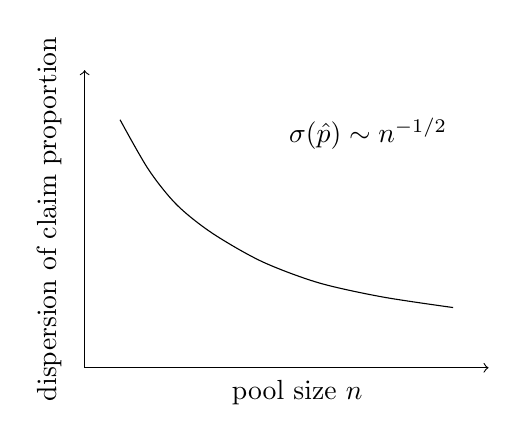
\begin{tikzpicture}[scale=0.9]
\draw[->] (0,0) -- (5.7,0);
\draw[->] (0,0) -- (0,4.2);
\draw plot[smooth] coordinates {(0.5,3.5) (0.9,2.8) (1.3,2.3) (1.8,1.9) (2.5,1.5) (3.3,1.2) (4.2,1.0) (5.2,0.85)};
\node at (3.0,-0.35) {pool size \(n\)};
\node[rotate=90] at (-0.5,2.1) {dispersion of claim proportion};
\node at (4.0,3.3) {\(\sigma(\hat p)\sim n^{-1/2}\)};
\end{tikzpicture}
\end{figure}

At this point in the lecture, however, Shiller immediately adds a warning. The formula is powerful, but it is not the whole institution. Insurance is not merely a theorem from probability theory. It is a human arrangement that can fail in many ways.

\section{Insurance as Institutional Design: Moral Hazard and Selection Bias}

The lecture's next move is one of the most important. Once the mathematics of pooling is on the table, Shiller refuses to leave it there. He asks what has to be done to make that mathematics operative in a real insurance company. The answer is: quite a lot.

First, contract design matters. The insurer has to specify what is covered and what is excluded. That is not a legal afterthought; it is part of the economic technology. If the contract is poorly written, the probabilistic logic will be undermined by strategic behavior or by disputes over what actually counts as a loss.

\begin{definition}
\emph{Moral hazard} is the effect of insurance on behavior when coverage changes the insured party's incentives in undesirable ways.
\end{definition}

The lecture's classic example is fire insurance on a house. If the policy creates a gain from destruction, then the whole institution becomes unstable. In a minimal notation, if \(V_{\text{house}}\) is the market value of the house and \(I_{\text{house}}\) is the insurance payment after destruction, then one basic design principle is
\begin{equation}
I_{\text{house}} < V_{\text{house}}.
\end{equation}
Shiller's verbal point is that if the insured still loses something after the fire, then there is no economic temptation to burn the house down. The same logic motivates exclusions for suspicious causes of death in life insurance.

\begin{definition}
\emph{Selection bias} in the lecture's language is the tendency for higher-risk individuals to seek coverage more aggressively than lower-risk individuals.
\end{definition}

If individuals know private information about their own risk and the insurer does not, then the composition of the insured pool becomes worse than the population from which it was drawn. In words, the lecture's mechanism is
\begin{equation}
\text{selection bias} \Longrightarrow \text{higher expected losses} \Longrightarrow \text{higher premiums} \Longrightarrow \text{exit of lower-risk buyers}.
\end{equation}
That spiral is why Shiller insists that real insurance requires not only a pooling model, but also underwriting, exclusions, screening, and a carefully defined proof of loss.

The lecture then expands the design problem into a list of institutional requirements:
\begin{itemize}
\item a contract that specifies covered and excluded risks;
\item a mathematical model of pooling, beginning with independence;
\item data, such as mortality tables, that let the insurer estimate risk;
\item a corporate or mutual form that determines who bears residual error;
\item government regulation, because policyholders may pay in for many years before discovering whether the company is sound.
\end{itemize}

\subsection{Question \& Answer}

\paragraph{Question.} If risk pooling works mathematically, why is insurance still hard to make reliable?

\paragraph{Answer.} Because pooling solves only the problem of random fluctuation under good conditions. It does not by itself solve incentive problems, informational asymmetries, contract ambiguity, weak data, poor organizational design, or lack of public trust. The institution must be engineered around the theorem.

Shiller's remark about regulation is especially important. In life insurance, the customer may pay premiums for a very long time and hope never personally to collect. That means trust cannot be built only by repeated short-run performance. Regulation is part of the design, not an external intrusion.

\section{AIG and the Failure of Independence}

The lecture next becomes concrete. Shiller turns to AIG, both because it had been the largest insurance company in the world and because Maurice ``Hank'' Greenberg was scheduled to visit the class. The historical details are not ornamental. They help explain why AIG was not a small fringe firm but a dominant institution with deep prestige and a long history.

The transcript is somewhat garbled on dates, but the central chronology is clear enough for the argument. AIG began in Shanghai in 1919, originally as American Asiatic Underwriters, under Cornelius Vander Starr. Greenberg later ran the company for decades. The larger pedagogical point is that this was a very large, seemingly sophisticated organization, not a naive startup that misunderstood elementary business.

The real mathematical issue appears only after this historical build-up. According to Shiller, AIG's failure came mainly from a failure of the independence assumption. The company became deeply exposed to real-estate risk through credit default swaps and mortgage-related securities. The working belief was that housing problems in one city would be offset by housing conditions elsewhere. In effect, the firm acted as though geographically dispersed housing risk would diversify.

But that logic depends on low dependence across exposures. When house prices fell nationally, the insurer did not face a set of nearly independent shocks. It faced a strongly aligned shock. In the language of the lecture,
\begin{equation}
\text{local housing weakness may diversify}, \qquad \text{national housing collapse does not.}
\end{equation}
The same pooling logic that works for many independent deaths or fires fails when one common factor moves many losses at once.

The federal government ultimately committed roughly \$182 billion to the rescue of AIG. Shiller is careful here: the bailout did not rescue shareholders in the ordinary sense. The shareholders lost most of their value, and the company later underwent a reverse split,
\begin{equation}
20 \text{ old shares} \mapsto 1 \text{ new share}.
\end{equation}
The firm survived, but the old equity was massively diluted and largely destroyed.

The deeper point is that AIG is not merely a crisis anecdote. It is the lecture's main warning about insurance mathematics. Pooling is powerful only to the extent that the risks really do offset one another. Once a common shock dominates, the insurance institution begins to look less like a stabilizing law of large numbers and more like a levered bet on one underlying state of the world.

\section{Guarantee Funds and the Architecture of Regulation}

After AIG, the lecture asks a new question. If insurance companies are regulated and if there are guarantee arrangements in place, why was a special bailout necessary? This question carries the lecture from firm failure into the architecture of the American system.

Shiller compares insurance protection to bank deposit insurance. Deposits are federally insured up to a limit, around \$250{,}000 at the time of the lecture. Insurance, however, is largely protected through state insurance guarantee funds. These are much more limited backstops, meant primarily for ordinary policyholders rather than for a gigantic, globally entangled firm like AIG. State limits of roughly \$500{,}000 in New York and Connecticut, and often around \$300{,}000 elsewhere, are nowhere near the scale of a systemic insurer with enormous financial counterparties.

\subsection{Question \& Answer}

\paragraph{Question.} If insurance already has guarantee funds, why did AIG still require a federal rescue?

\paragraph{Answer.} Because the guarantee funds are small, state-based protections for ordinary policyholders, not system-wide facilities capable of absorbing the collapse of a gigantic firm whose failure could destabilize banks, counterparties, and markets. AIG was not only an insurance company with policies outstanding; it was also a node in the broader financial system.

This leads into the distinctive U.S.\ regulatory structure. Under the McCarran--Ferguson Act of 1945, insurance regulation remained primarily a state matter. The consequence is fragmentation: an insurer operating nationally faces many state regulators rather than one national supervisor. The National Association of Insurance Commissioners helps standardize practice, but it is a coordinating body rather than a sovereign national regulator.

Dodd--Frank then appears in the lecture as a limited federal response to the AIG lesson. Shiller's point is not that the United States suddenly nationalized insurance regulation. It did not. Rather, the federal government created a mechanism to monitor insurance companies for \emph{systemic risk}. If an insurer begins to look like another AIG, federal bodies may become involved.

The mathematical lesson from earlier sections reappears here in institutional form. The federal government is not intervening because it discovered that the law of large numbers is false. It is intervening because real institutions may build pools whose dependence structure is much worse than their own models admit.

\section{Types of Insurance, Health Insurance, and New Risk Management}

Only after the crisis and regulatory architecture are laid out does the lecture return to the taxonomy of insurance. Life insurance is the largest private category in the lecture's numbers, followed by health insurance and then property and casualty insurance. Shiller mentions term insurance, whole life, variable life, and annuities, but does not dwell on taxonomy for its own sake. The main point is that these are all inventions: different contractual ways of organizing the transfer of risk.

Health insurance then becomes the main institutional example, because it exposes the same problems of pooling, information, and incentives in a more publicly visible form. Many countries addressed these problems by adopting national systems. The United States, by contrast, retained a stronger private-insurance tradition and therefore encountered persistent failures of participation and incentive design.

The lecture's health-insurance logic is a direct extension of the earlier analysis of selection bias. If healthy people stay out of the pool while sick people enter, then premiums rise and the system becomes unstable. This is why the 2010 reforms use penalties and exchanges rather than relying on purely voluntary participation. In the lecture's causal language,
\begin{equation}
\text{mandatory entry of healthy people} \Longrightarrow \text{broader pool} \Longrightarrow \text{lower average cost per insured} \Longrightarrow \text{lower premiums}.
\end{equation}
The approximately \$700 penalty for remaining uninsured is part of that design. It is not a side tax. It is an attempt to change the composition of the pool.

Shiller also revisits moral hazard on the provider side. In a fee-for-service system, doctors may have an incentive to order procedures rather than preserve long-run health. The HMO is introduced as a design response: pay doctors salaries rather than per procedure, and the incentive to over-treat is reduced. The Yale Health Plan then appears as a local example of this structure.

EMTALA, by contrast, is presented as an unfunded mandate. Hospitals must provide emergency treatment, but the law does not itself solve the financing problem. The result is not a clean insurance system, but a hybrid in which treatment is required while payment remains uncertain and often produces debt. Again the lecture returns to the same theme: the institution only works if the incentives and financing rules line up.

The lecture's closing examples widen the scope. Haiti illustrates what happens when disaster risk is scarcely insured at all. The loss is not merely uncompensated afterward; the absence of insurance also means weaker ex ante discipline over construction standards. Katrina shows a different problem. Insurance existed, but the contract definition of the loss became difficult because hurricane damage combined wind and flood. The dispute was not over whether there had been a disaster. It was over which disaster had occurred for contractual purposes.

Terrorism insurance pushes the same logic into a more extreme domain. Traditional policies exclude war and terrorism because these are highly correlated risks. A terrorist event is not the sort of isolated claim that pooling handles comfortably. TRIA therefore appears as a public-private arrangement in which private insurers must offer terrorism coverage, while the government stands behind a portion of truly extreme losses.

Finally, catastrophe bonds extend the reach of insurance by moving catastrophic risk into broader capital markets. The lecture's Mexican example is best stated cautiously, since some figures in the transcript may be noisy, but the structure is clear. The bond is designed so that investors bear loss if a specified catastrophe occurs. In that sense the instrument is insurance-like, but it is issued and traded as a financial security. The risk is spread over global portfolios rather than concentrated on the balance sheet of one government or one insurer.

\section{Summary}

The lecture begins with a simple claim and ends by deepening it. Insurance belongs inside finance because it is a risk-management institution. Its mathematical core is pooling, and under independence the volatility of the claim proportion falls like \(1/\sqrt{n}\). That is why insurance can work at all.

But the lecture's real achievement is to show that this mathematical insight is only the beginning. Contracts must limit moral hazard. Pools must be protected against selection bias. Loss definitions must be precise. Data must be gathered. Firms must be organized. Regulators must monitor them. And when the independence assumption fails, as in AIG or in war and terrorism risk, the institution may require new public structures or new financial instruments.

So insurance emerges here not as a settled branch of administration, but as an unfinished technology. It already protects health, families, homes, and businesses. Yet it still struggles with systemic dependence, changing probabilities, inflation, underinsurance in poorer countries, and the hard design problem of getting people and institutions to do the right thing before the loss occurs.